% !TEX root = main.tex
\section{Theory}

\subsection{Bridge Weigh-in-Motion}
A Bridge Weigh-in-Motion system is based on measurements of a bridge's deformation. The BWIM system uses these measurements to calculate passing vehicles axle loads.
There are different approaches to assembling such a system, but they typically consists of a strain gauge measuring the strain induced by passing vehicles, a axle detector used to find the vehicle speed and spacing of axles and a computer or data storage device. An algorithm then is able to use the data gathered from the axle detector and strain gauge to calculate axle loads \cite{Quilligan}.
\subsubsection{Moses' Algorithm}
Moses' algorithm is based on the fact that a moving load along a bridge will set up stresses in proportion to the product of the value of the influence line and the axle load magnitude. The influence line being defined as the bending moment at the point of measurement due to a unit axle load crossing the bridge \cite{Quilligan}.

Moses' algorithm is built from the fact that a moving unit load on a bridge will induce stresses proportional to the product of the value of the influence line and the axle load magnitude.

Each individual girder's stress is related to moment:
\begin{equation}
\overbrace{\sigma_{i}}^\text{stress in i'th girder} = \frac{\overbrace{M_i}^\text{bending moment i'th girder}}{\underbrace{W_i}_\text{section modulus}}
\end{equation}
Expressing the moment in terms of strain gives
\begin{equation}
M_i = W_i \sigma_i = \overbrace{E}^\text{Modulus of elasticity} \times W_i \times \underbrace{\varepsilon_i}_\text{strain in i'th girder}
\end{equation}
The sum of the individual girder moments is therefore:
\begin{equation}
M = \sum_{i = 1}^{N} M_i = \sum_{i = 1}^{N} EW_i \varepsilon_i = EW \sum_{i = 1}^{N} \varepsilon_i
\label{equation:moment_strain}
\end{equation}
The sum of the girder strains is proportional to the gross bending moment. The total bending moment and the measured strain is thus directly related by $EW$. These constants can be calculated through the bridge's dimensions and material properties. However through measuring the effects of a known vehicle passing the bridge these constants can be derived.

Weigh in motion is an inverse type problem, the strain is measured and the cause of the strain is to be calculated. The theoretical bending moment corresponding to axle loads on the bridge at one strain sample, is given by:
\begin{equation}
M_k^T = \sum_{i = 1}^{N} A_i I_{(k-C_i)}
\label{equation:theoretical_strain}
\end{equation}
\begin{equation}
C_i = (L_i \times f)/v
\end{equation}
Where:
\begin{description}
	\item N = \textit{the number of vehicle axles}
	\item $A_i = $ \textit{the weight of axle i}
	\item $I_{k-C_i} = $ \textit{the influence line ordinate for axle i at sample k}
	\item $L_i$ = the distance between axle i and the first axle in meters
	\item $C_i$  = \textit{The number of strain samples corresponding to the axle distance $L_i$}
	\item f = the strain gauge's sampling frequency, in \SI{}{\Hz}
\end{description}

\subsection{Influence lines}
For a B-WIM system the influence line is defined as "the bending moment at the point of measurement due to a unit axle load moving along the bridge \cite{bwim_an_overview}". The influence line could be found through assembling a model of the bridge in any CAD or frame-program, this would however take a lot of time especially for more advanced bridge's. Depending on the support of the bridge the influence lines takes different theoretical forms, as seen in Figure \ref{fig:theoreticalInfl}. The true influence line for a bridge lie somewhere in between the simply supported and fixed version \cite[p.~146]{bwim_an_overview}.
Influence lines is a big source of error in a B-WIM system.
\begin{figure}[h]
\centering
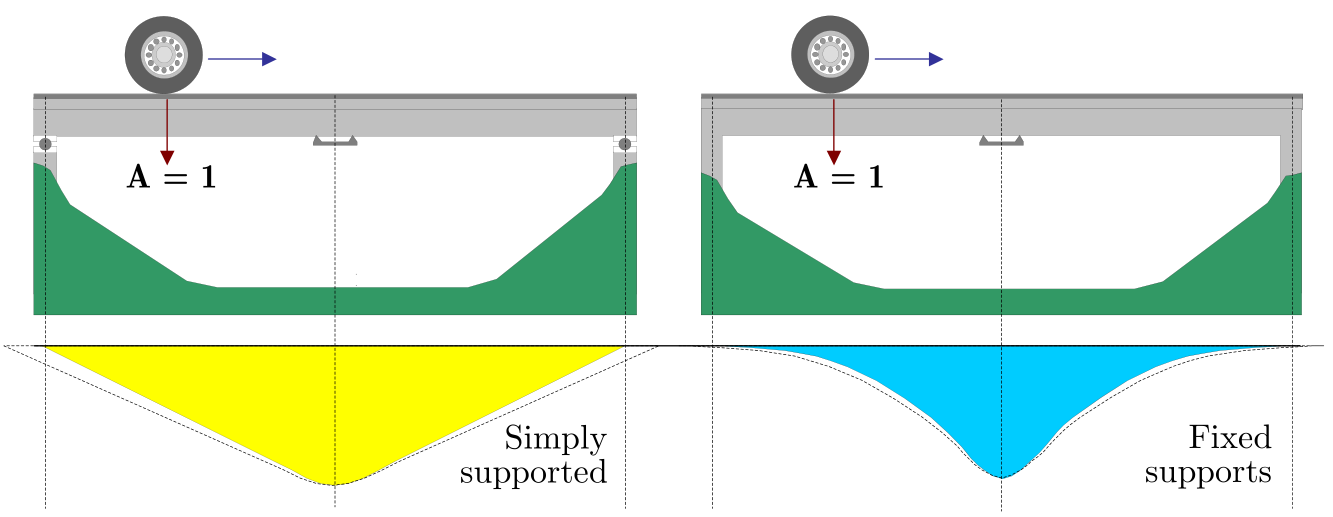
\includegraphics[scale=0.5]{figures/inflLinesQuilligan}
\caption{Influence lines for simply and fixed supported bridges, figure from \cite{Quilligan}}
\label{fig:theoreticalInfl}
\end{figure}

Znidaric and Baumgärter \cite{bwim_an_overview}, did a study on the effect of choice of influence line. This study shows errors up to 10\% for a short \SI{2}{\metre} bridge span and errors of several hundred percent for a \SI{32}{\metre} bridge span. This underlines the importance of using correct influence lines for a B-WIM system.
\begin{figure}[h]
\centering
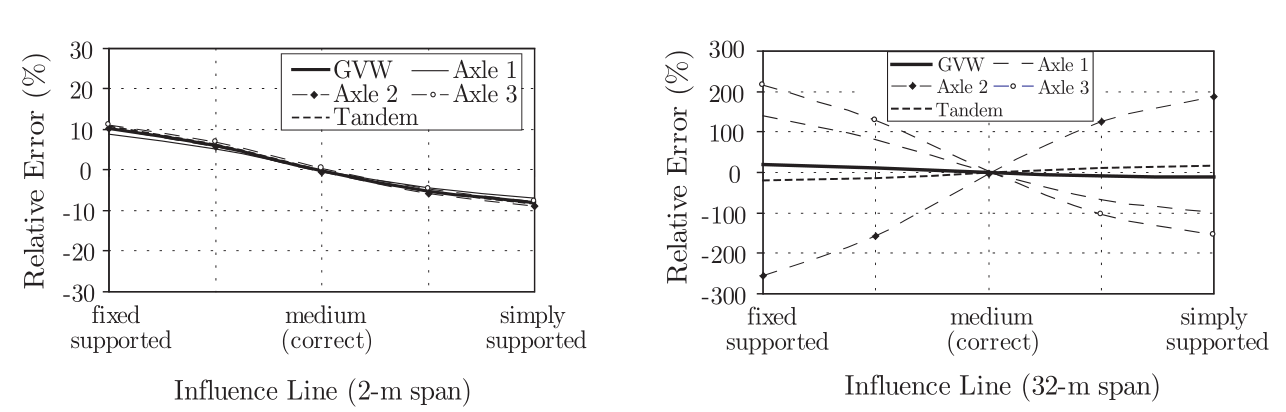
\includegraphics[scale=0.5]{figures/error_in_weights_dueTo_infl}
\caption{Errors of axle loads due to wrongly selected influence lines, figure from \cite{Quilligan}}
\label{fig:errorOfInfl}
\end{figure}
\subsubsection{Matrix method}
Quilligan \cite{Quilligan} developed a 'matrix method' to calculate the influence line of a bridge through the measured strain induced by a vehicle. This method is derived from Moses', equation \ref{equation:moses}.
\begin{equation}
Error = \sum_{k = 1}^{K} [\varepsilon_{k}^{measured} - \varepsilon_{k}^{theoretical}]^2
\label{equation:moses}
\end{equation}
Equation \ref{equation:moses} were originally used to filter out the dynamic response of the bridge.
The theoretical strain in this equation can be expressed as a product of axle loads and influence ordinates at sampling points, see equation \ref{equation:theoretical_strain}, thus we can expand equation \ref{equation:moses}:
\begin{equation}
Error = \sum_{k = 1}^{K} \Big[\varepsilon_{k}^{measured} - \Big(\sum_{i = 1}^{N} A_i I_{(k-C_i)}\Big)\Big]^2
\label{equation:moses_expanded}
\end{equation}
The set of influence ordinates $I$ that minimizes $Error$, forms the wanted influence line.
\begin{equation}
\frac{\partial Error}{\partial I_R} = \frac{\partial \sum_{k = 1}^{K} \Big[\varepsilon_{k}^{measured} - \Big(\sum_{i = 1}^{N} A_i I_{(k-C_i)}\Big)\Big]^2}{\partial I_R}
\end{equation}
For a given number of known axle loads this equation comes down to a set of $(K - C_n)$ number of linear equations. Rearranging the equations and writing them in matrix form leads to:
\begin{equation}
\begin{bmatrix} AxleMatrix \end{bmatrix}_{K-C_N, K-C_N} \begin{Bmatrix} I \end{Bmatrix}_{K-C_N, 1} = \begin{Bmatrix} M \end{Bmatrix}_{K-C_N, 1}
\label{equation:matrixForm}
\end{equation}
Where:
\begin{description}
\item $\begin{Bmatrix} M \end{Bmatrix}$ = a vector depending on axle weights and measured strain, $M_{i, 1} = \Big(\sum_{j = 1}^{N} A_j \varepsilon_{(i+C_j)}\Big)$
\item $\begin{bmatrix} AxleMatrix \end{bmatrix}$ is a matrix depending only on the axle loads, defined by equation \ref{axleMatrix}.
\end{description}
\begin{equation}
\begin{bmatrix} AxleMatrix \end{bmatrix} = \sum_{i = 1}^{N} \sum_{j = i}^{N} \begin{bmatrix} AxleMatrix \end{bmatrix} + \big( A_i A_j  \begin{bmatrix} Diagonal \end{bmatrix}_{C_j - C_i}\big)
\label{axleMatrix}
\end{equation}
Which produces the upper triangle of the symmetric AxleMatrix.
Where:
\begin{description}
\item $\begin{bmatrix} Diagonal \end{bmatrix}_{C_j - C_i}$ = a diagonal matrix of ones, where diagonal is placed with an offset, $C_j - C_i$, from the center matrix diagonal.
\end{description}
Solving equation \ref{equation:matrixForm} for the influence ordinate vector gives the influence line for the strain history. This can be done through inversion of the AxleMatrix (equation \ref{axleMatrix}) or other numerical solutions like a Cholesky factorization.
\subsubsection{Optimization}
testing \cite{Liljencrantz}.
For this thesis one of the goals where to assess the accuracy of and optimization algorith for finding a bridges influence lines. To develope such an algorithm test strain signal where produced by a matlab script, and the algorithm developed was to find the influence line used to produce the strain signal.
In theory using optimization to identify influence lines should work well, and indeed it did for these produced theoretical strain signals. 

\subsection{Finding the train's speed}

\subsection{The axle distances}
